\noindent
\paragraph{Grundlagen}\mbox{}\\
\paragraph{Symbole}\mbox{}\\
\begin{tabularx}{\columnwidth}{@{}X|X@{}}
    \hline
    $\exists$: Existiert mind. 1 & $\exists!$: Existiert genau 1 \\ \hline
    $\nexists$: Existiert nicht  & $\forall$: Für alle           \\ \hline
\end{tabularx}
\vspace{1mm}

\noindent
\textit{Menge und Elemente gemäss CANTOR}\linebreak
\begin{itemize}
    \item Unter eine Menge verstehen wir jede Zusammenfassung von bestimmten wohlunterschiedenen Objekten (Elemente) unserer Anschauung oder unseres Denkens zu einem Ganzen.
    \item Sei $A$ eine Menge und $x$ ein $Element$ von $A$. Die Aussage, dass $x$ ein $Element$ von $A$ ist, wird geschrieben gemäss: \fbox{$x \in A$}
    \item Verneinung: \fbox{$x \notin A$}
    \item Leere Menge: \fbox{$ \varnothing = \{\} $}
    \item Menge A besteht aus Elementen von Grundmenge G, bei welchen Elemente gegebene Kriterien erfüllenn:
    \item $A = \{x \in G\,|\,x$ hat die Eigenschaften...$ \}$
    \item Bsp für N. Zahlen von 1 bis 4: $A = \{x \in \mathbb{N} \,|\,1 \leq  x \leq  4 \}$
    \item Teilmenge: \fbox{$A \subseteq B \leftrightarrow (x \in A \rightarrow x \in B) $}
    \item Strikte Teilmenge: \fbox{$A \subset B \leftrightarrow (A \subseteq B \land A \neq B) $}
    \item Verneinung Teilmenge: $\nsubseteq$
    \item Verneinung Strikte Teilmenge: $\not\subset$
\end{itemize}
\vspace{1mm}

\noindent
\textit{Mengenoperationen}\linebreak
\begin{itemize}
    \item Vereinigung: $A \cap B := \{x\,|\,x \in A\, \lor\, x \in B \}$
    \item 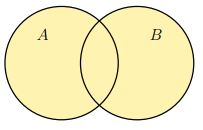
\includegraphics[width=50pt]{./images/vereinigung.jpg}
    \item Schnittmenge: $A \cup B := \{x\,|\,x \in A\, \land\, x \in B \}$
    \item 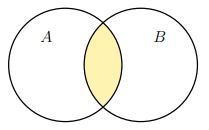
\includegraphics[width=50pt]{./images/schnittmenge.jpg}
    \item Differenz: $A \backslash B := \{x\,|\,x \in A\, \land\, x \notin B \}$
    \item 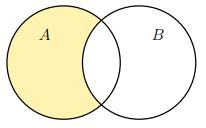
\includegraphics[width=50pt]{./images/differenz.jpg}
    \item Symmetrische Differenz: $A\Delta B := (A\backslash B)\cup (B\backslash A)$
    \item 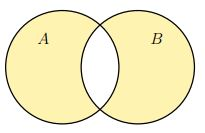
\includegraphics[width=50pt]{./images/systematische_differenz.jpg}
    \item Komplementierung (G Grundmenge): $\overline{A} := G\backslash A$
    \item 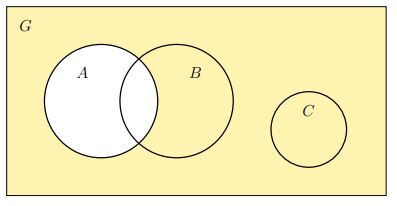
\includegraphics[width=80pt]{./images/komplementaer.jpg}
\end{itemize}
\vspace{1mm}

\paragraph{Mengen Rechenregeln}\mbox{}\\
\begin{tabularx}{\columnwidth}{@{}X|X@{}}
    \hline
    $B\cup A = A\cup B$                                              & $B\cap A = A \cap B$                                                      \\ \hline
    $(A\cup B)\cup C = A\cup (B\cup C)$                              & $(A\cap B)\cap C = A\cap (B\cap C)$                                       \\ \hline
    $A\cap (B\cup C) = (A\cap B)\cup (A\cap C)$                      & $A\cup (B\cap C) = (A\cup B)\cap (A\cup C)$                               \\ \hline
    $A\cup (A\cap B) = A$                                            & $A\cap (A\cup B) = A$                                                     \\ \hline
    $(A\backslash B)\backslash C = A \backslash (B\cup C)$           & $A\backslash (B\backslash C) = (A \backslash B)\cup (A\cap C)$            \\ \hline
    $(A\cup B) \backslash C = (A \backslash C) \cup (B\backslash C)$ & $(A\cap B) \backslash C = (A \backslash C) \cap (B \backslash C)$         \\ \hline
    $A\backslash (B\cup C) = (A \backslash B)\cap (A \backslash C)$  & $ A\backslash(B\cap C) = (A\backslash B) \cup (A \backslash C) $          \\ \hline
    $B\Delta A = A\Delta B$                                          & $(A\Delta B)\Delta C = A\Delta (B\Delta C)$                               \\ \hline
    $(A\Delta B)\cap C = (A\cap C)\Delta (B\cap C)$                  &                                                                           \\ \hline
    $\overline{A\cup B} = \overline{A}\cap \overline{B}$             & $\overline{A\cap B} = \overline{A}\cup \overline{B}$                      \\ \hline
    $\overline{A\cup B} = G\backslash (A\cup B) =$                   & $ = (G\backslash A) \cap (G\backslash B) = \overline{A}\cap \overline{B}$ \\ \hline
    $\overline{A\cap B} = G\backslash (A\cap B) =$                   & $ = (G\backslash A) \cup (G\backslash B) = \overline{A}\cup \overline{B}$ \\ \hline
\end{tabularx}
\vspace{1mm}

\noindent
\textit{Kartesisches Produkt}\linebreak
\fbox{$A\, \times B := \{(x;y)\, |\, x \in A\, und\, y \in B\}$}
\vspace{1mm}

\paragraph{Zahlenmenge}\mbox{}\\
\begin{tabularx}{\columnwidth}{@{}X|X@{}}
    \hline
    $\mathbb{N}$: natürlichen Zahlen & $\mathbb{N}_0$: natürlichen Zahlen mit die Zahl 0 \\ \hline
    $\mathbb{Z}$: ganze Zahlen       & $\mathbb{Q}$: rationale Zahlen                    \\ \hline
    $\mathbb{R}$: reelle Zahlen      & $\mathbb{C}$: Komplexe Zahlen                     \\ \hline
\end{tabularx}
\vspace{1mm}

\paragraph{Intervalle}\mbox{}\\
\begin{tabularx}{\columnwidth}{@{}X|X@{}}
    \hline
    [a,b] = $\{x \in \mathbb{R} | a \leq  x \leq b \}$ & ]a,b] = $\{x \in \mathbb{R} | a < x \leq b \}$ \\ \hline
    [a,b[ = $\{x \in \mathbb{R} | a \leq  x < b \}$    & ]a,b[ = $\{x \in \mathbb{R} | a < x < b \}$    \\ \hline
    $\mathbb{R}^{+}_0 = [0,\infty]$                    & $\mathbb{R}^{+} = ]0,\infty]$                  \\ \hline
\end{tabularx}
\vspace{1mm}

\paragraph{Körperaxiome}\mbox{}\\
\noindent
Addition\linebreak
\begin{tabularx}{\columnwidth}{@{}X|X@{}}
    \hline
    Assoziativgesetz      & $x+(y+z) = (x+y)+z$                                                  \\ \hline
    Kommutativgesetz      & $x+y = y+x$                                                          \\ \hline
    Existenz der Null     & $\exists$ eine Zahl 0 $\in \mathbb{R}$:\linebreak $0+x=x, \forall x$ \\ \hline
    Existenz der Negation & $\forall x\exists -x$: $x+(-x) = 0$                                  \\ \hline
\end{tabularx}
\vspace{1mm}
\noindent
Multiplikation\linebreak
\begin{tabularx}{\columnwidth}{@{}X|X@{}}
    \hline
    Assoziativgesetz      & $x*(y*z) = (x*y)*z$                               \\ \hline
    Kommutativgesetz      & $x*y = y*x$                                       \\ \hline
    Existenz der Eins     & $\exists (1\in \mathbb{R}) \land 1 \neq 0: 1*x=x$ \\ \hline
    Existenz der Inversen & $\forall x \neq 0, \exists x^{-1}: x*x^{-1}=1$    \\ \hline
    Distributivgesetz     & $x*(y+z) = x*y + x*z = 1$                         \\ \hline
\end{tabularx}
\vspace{1mm}

\paragraph{Funktionen}\mbox{}\\
\begin{tabularx}{\columnwidth}{@{}X|X@{}}
    \hline
    $f : A \rightarrow B$                           & $x \rightarrow f(x) := Kondition$   \\ \hline
    $f : \{3,4\} \rightarrow \{5,6,7\}$             & $x \rightarrow f(x) := x + 2$       \\ \hline
    $f$: Funktionsname                              & $A$: Definitionsmenge               \\ \hline
    $B$: Zielmenge                                  & $x$: unabhängige Variable, Argument \\ \hline
    $f(x)$: abhängige Variable, Funktionswert                                             \\ \hline
    $f(y)^{-1}: Umkehrfunktion$                                                           \\ \hline
    Identität ist die Funktion zwischen zwei Mengen & $id_A : B \rightarrow A$            \\ \hline
\end{tabularx}
\vspace{1mm}

\paragraph{Bild und Urbild}\mbox{}\\
Seien A und B zwei Mengen, $f: A \rightarrow B$ eine Funktion und $\overline{A} \subseteq A$ sowie $\overline{B} \subseteq B$.
\begin{itemize}
    \item Bild: $f(\overline{A}) \subseteq B$
    \item Urbild: $f^{-1}(\overline{B}) \subseteq A$
\end{itemize}
\vspace{1mm}

\paragraph{Surjektiv}\mbox{}\\
\begin{itemize}
    \item Zu jedem $y\in B$ aus dem Zielbereich mindestens ein $x\in A$ aus dem Definitionsbereich
    \item f heisst surjektiv: $\forall y \in B, \forall x \in A$
    \item $y= f(x)$
    \item Beweis: $y = f(x)$
    \item 1. Nach x auflösen
    \item 2. Ausdruck hängt von y ab
    \item 3. Überprüfen, ob dieser Ausdruck für alle y aus $y\in B$ definiert ist und ein Teil von A ist
\end{itemize}
\vspace{1mm}

\paragraph{Injektiv}\mbox{}\\
\begin{itemize}
    \item Für jedes Element $y\in B$ höchstens ein Element $x\in A$ wobei $f(x)=y$
    \item Annahme: $f(x_1) = f(x_2)$, Ziel: $x_1 = x_2$
\end{itemize}
\vspace{1mm}

\paragraph{Reihen und Folgen}\mbox{}\\
\begin{itemize}
    \item \fbox{$a: \mathbb{N}\rightarrow B$,  $n \rightarrow a(n)$}
    \item Arithmetische Folge, $\forall c \in \mathbb{R},$ so dass $\forall k \in \mathbb{N}^{+}$
    \item $a_{k+1} = a_{k} + c$
    \item Geometrische Folge, $\forall c \in \mathbb{R},$ so dass $\forall k \in \mathbb{N}^{+}$
    \item $a_{k+1} = a_{k} * c$
    \item Arithmetische Folge ist die diskrete Version einer linearen Funktion:
    \item $a_n = a_0 + c * n$
    \item Geometrische Folge ist die diskrete Version einer Exponentialfunktion:
    \item $a_n= a_0 * c^n$ \\
\end{itemize}
\vspace{1mm}

\paragraph{Beschrankte Folgen}\mbox{}\\
\begin{itemize}
    \item Oben beschränkt: \fbox{$a_n \leq a_O$}
    \item Unten beschränkt: \fbox{$a_n \geq a_U$}
    \item Die folge $a_n$ heisst beschränkt wenn: \fbox{$a_n \in [a_U,a_O]$}
\end{itemize}
\vspace{1mm}

\paragraph{Monotone Folgen}\mbox{}\\
\begin{itemize}
    \item Monoton steigend: \fbox{$a_{k+1} \geq a_k $}
    \item Monoton streng steigend: \fbox{$a_{k+1} > a_k $}
    \item Monoton fallend: \fbox{$a_{k+1} \leq a_k $}
    \item Monoton streng fallend: \fbox{$a_{k+1} < a_k $}
\end{itemize}
\vspace{1mm}

\paragraph{Monotonie untersuchen}\mbox{}\\
\begin{itemize}
    \item Um eine Folge auf Monotonie zu untersucen, kann man die Folgeglieder der Differenzenfolge gegen Null abschätzen
    \item \fbox{$d_n := a_{n+1} - a_{n}$}
    \item Resultat interpretieren:
    \item $d_n \geq 0 \leftrightarrow a_{n+1} \geq a_n \leftrightarrow a_n$ ist monoton steigend
    \item $d_n > 0 \leftrightarrow a_{n+1} > a_n \leftrightarrow a_n$ ist streng monoton steigend
    \item $d_n \leq 0 \leftrightarrow a_{n+1} \leq a_n \leftrightarrow a_n$ ist monoton fallend
    \item $d_n < 0 \leftrightarrow a_{n+1} < a_n \leftrightarrow a_n$ ist streng monoton fallend
\end{itemize}
\vspace{1mm}